\documentclass[10pt]{article}
\usepackage{graphicx}
\usepackage{xeCJK}
\usepackage{placeins}
\usepackage{float}
\usepackage{amsmath}
\setCJKmainfont{MS Mincho} % for \rmfamily
\setCJKsansfont{MS Gothic} % for \sffamily
\graphicspath{ {../image/} }
\renewcommand{\figurename}{図}
\renewcommand{\tablename}{表}

\title{Assignement 4}

\author{Phusaeng Natthaphat (04B23054)}
\date{2026年4月30日}


\begin{document}

\maketitle

\section{section}
　Langevin 方程式を解析的に解いてみる。
\begin{equation}\label{eqn:Langevin}
    \begin{split}
        m\frac{d}{dt}\mathbf{v}(t)&=-\zeta\mathbf{v}(t)+\mathbf{F}_{\text{B}}(t)\\
        \langle\mathbf{F}_{\text{B}}(t)\cdot\mathbf{F}_{\text{B}}(t')\rangle&=2d\zeta k_BT\delta(t-t')
    \end{split}
\end{equation}
$d$はベクトルの次元である。ただし、$\langle\ldots\rangle$は何らかの平均を取る動作とする。\\
　$\mathbf{v}(t)$の一般解は式\ref{eqn:solution}から次である。
\begin{equation}
    \mathbf{v}(t)=e^{-\frac{\zeta}{m}t}\mathbf{v}(0)+\frac{1}{m}\int_{0}^{t}e^{-\frac{\zeta}{m}(t-t')}\mathbf{F}_\text{B}(t')dt'
\end{equation}
\hspace*{\parindent} The first term contains initial information of the particle, while the second term describe the overall effect of randomness on
particle's dynamic. After long enough time $t$ passes, the first term decays exponentially, leaving only the randomness contribution.
\begin{equation}\label{eqn:v_longtime}
    \mathbf{v}(t)\sim\frac{1}{m}\int_{0}^{t}e^{-\frac{\zeta}{m}(t-t')}\mathbf{F}_\text{B}(t')dt'
\end{equation}
\hspace*{\parindent} In the following analysis we restrict ourselves to only investigate the long term behaviour of particle, such that we will
repeatly use (\ref{eqn:v_longtime}).\\ \hspace*{\parindent}
One significant remark to be made is, the information about initial conditions of the Langevin equaiton is lost under
long time (steady state) behavior. This initial conditions-independence will play a crucial role in the simulation, because we don't have to specify
the initial conditions of each particle, we can make an ensemble of particles out of one long string of i.i.d. random process.

Here I took some liberty to define Auto Correlation Function $C(t_1,t_2)$.
\begin{equation}\label{eqn:C_def}
    C(t_1,t_2)=\langle\mathbf{v}(t_1)\cdot\mathbf{v}(t_2)\rangle
\end{equation}
$C(t_1,t_2)$の解析解を求めよう。I will follow the proof in Lecture note; however, some mathematical/physical remarks will be made and discussed along the derivation.
First, take dot product of (\ref{eqn:Langevin}) with $\mathbf{v}(t_2)$ and take the average $\langle\ldots\rangle$.
\begin{equation}
    \begin{split}
        m\dfrac{d}{dt}\langle\mathbf{v}(t)\cdot\mathbf{v}(t_2)\rangle&=-\zeta\langle\mathbf{v}(t)\cdot\mathbf{v}(t_2)\rangle+\langle\mathbf{F}_\text{B}(t)\cdot\mathbf{v}(t_2)\rangle
    \end{split}
\end{equation}
I implicitly assume that time differential operator $d/dt$ and average operator $\langle\ldots\rangle$ can be exchanged order.
The second term is 0 because velocity at time $t=0$ has no correlation with random fluctuation at time $t$. This is purely physical constrain made and can not be mathematically formulated properly,
because we didn't give the exact formula of $\langle\ldots\rangle$.\\ \hspace*{\parindent}
Subsitute $C(t)$ back to get the differential equation of $C(t)$
\begin{equation}\label{eqn:C_ODE}
    \dfrac{d}{dt}C(t)=-\dfrac{\zeta}{m}C(t)
\end{equation}
The solution is obvious,
\begin{equation}
    C(t)=C(0)e^{-\zeta t/m}
\end{equation}
(\ref{eqn:C_ODE}) has time translation symmetry i.e. by applying transformation $T_\varepsilon:t\mapsto t+\varepsilon$ to $C(t)$, the transformed $C'(t)=T_\varepsilon C(t)=C(t+\varepsilon)$ is still solution of (\ref{eqn:C_ODE}).



$\Delta \mathbf{r}(t)$は次のように定義する。
\begin{equation}
    \Delta \mathbf{r}(t):=\mathbf{r}(t)-\mathbf{r}(0)=\int_{0}^{t}\mathbf{v}(t')dt'
\end{equation}

第2，3項が消えるなぜならば、$\mathbf{v}(0)$と$\mathbf{F}_\text{B}(t)$は無関係である。

最終的に
\begin{equation}\label{eqn:MSD}
    \langle\Delta\mathbf{r}(t)^2\rangle=\dfrac{2dk_BT}{\zeta}\left\{t+\dfrac{m}{\zeta}e^{-\zeta t/m}-\dfrac{m}{\zeta}\right\}
\end{equation}
と証明できた。これを無次元化する。
\begin{equation}
    \begin{split}
        \Delta \mathbf{r}&=a\Delta\tilde{\mathbf{r}}\\
        t&=t_0\tilde{t}=\dfrac{m}{\zeta}\tilde{t}
    \end{split}
\end{equation}
式\ref{eqn:MSD}は次の形をする。
\begin{equation}
    \begin{split}
        \langle\Delta\tilde{\mathbf{r}}(\tilde{t})^2\rangle&=2d\dfrac{k_BTm}{a^2\zeta}\left\{\tilde{t}+e^{-\tilde{t}}-1\right\}\\
        :=&2dT^*\left\{\tilde{t}+e^{-\tilde{t}}-1\right\}
    \end{split}
\end{equation}

\section{結果}
Mean Square Displacement (MSD)の時間変化は以下である(図\ref{fig:MSD})。
\begin{figure}[H]
    \centering
    \makebox[\textwidth][c]{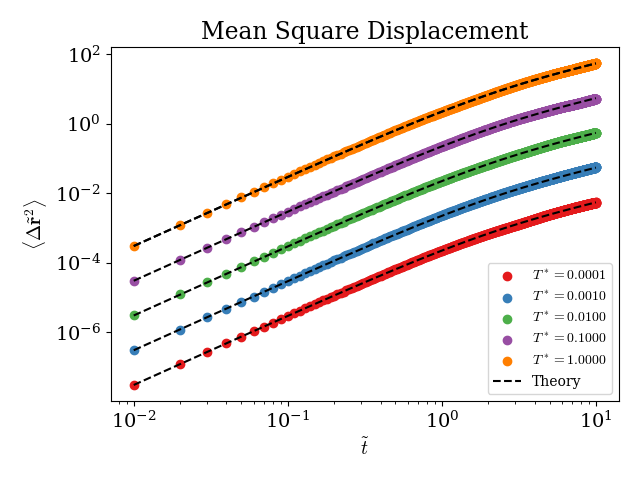
\includegraphics[width=\textwidth]{MSD.png}}
    \caption{Mean Square Displacment}
    \label{fig:MSD}
\end{figure}
また、Auto Correlation Functionのグラフは以下である(図\ref{fig:AutoCorrelation})。
\begin{figure}[H]
    \centering
    \makebox[\textwidth][c]{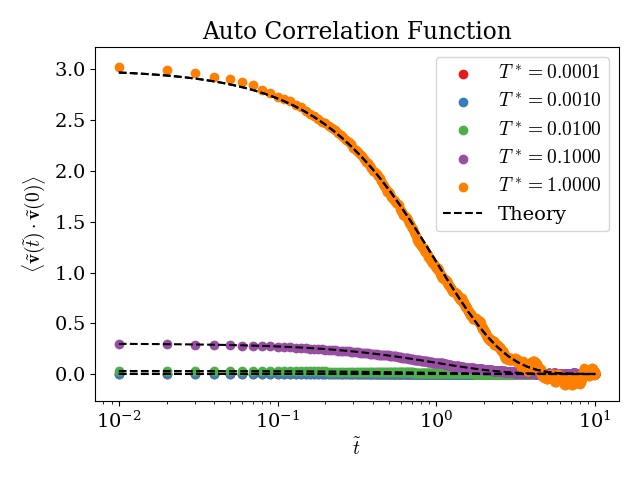
\includegraphics[width=\textwidth]{Correlation.png}}
    \caption{Mean Square Displacment}
    \label{fig:AutoCorrelation}
\end{figure}
図からわかるようにMSDのシムレイション結果が理論値とよく合っている。一方、Auto Correlation Funcitonの
シムレイション結果は時間が経つにつれて、理論値から離れていく。

\section{Appendix}
\begin{equation}\label{eqn:general}
    \dot{x}(t)=ax(t)+b(t)
\end{equation}
の一般解を求めよう。まず
\begin{equation}
    x(t)=e^{at}y(t)
\end{equation}
とおく。式\ref{eqn:general}が
\begin{equation}
    \dot{y}(t)=e^{-at}b(t)
\end{equation}
となり、
\begin{equation}
    y(t)=y(0)+\int_{0}^{t}e^{-at'}b(t')dt'
\end{equation}
だと分かる。すなわち、式\ref{eqn:general}の一般解が
\begin{equation}\label{eqn:solution}
    x(t)=e^{at}x(0)+\int_{0}^{t}e^{a(t-t')}b(t')dt'
\end{equation}
である。

\end{document}